% Author: Paula García-Molina
% Journal: New Journal of Physics (NJP)
\documentclass[12pt]{iopart}
\usepackage{iopams}
\usepackage[utf8]{inputenc}
\usepackage[english]{babel}
\usepackage{float} % Placement of figures
\usepackage{hyperref}
\usepackage{braket} % Braket notation
\usepackage{bm} % Bold symbols
% \usepackage{amsmath} %eqref and more
\usepackage{xcolor} % Color
\usepackage{tikz} % Figures in latex
\usepackage{amssymb} % \leqslant
\pdfminorversion=4

% These are missing from the IOP template
\newcommand{\eqref}[1]{(\ref{#1})}

\newcommand{\comm}[1]{\textbf{\textcolor{red}{#1}}}

\begin{document}

\title{Global optimization of MPS in quantum-inspired numerical analysis}

\author{Paula García-Molina}
\address{Institute of Fundamental Physics IFF-CSIC, Calle Serrano 113b, Madrid 28006, Spain}
\ead{paula.garcia@iff.csic.es}

\author{Luca Tagliacozzo}
\address{Institute of Fundamental Physics IFF-CSIC, Calle Serrano 113b, Madrid 28006, Spain}

\author{Juan José García-Ripoll}
\address{Institute of Fundamental Physics IFF-CSIC, Calle Serrano 113b, Madrid 28006, Spain}
\vspace{10pt}
% \begin{indented}
% \item[]June 2022
% \end{indented}

\begin{abstract}
This work discusses the solution of partial differential equations (PDEs) using matrix product states (MPS). The study focuses on the search for the lowest eigenstates of a Hamiltonian equation, for which five algorithms are introduced: imaginary-time evolution, steepest gradient descent, an improved gradient descent, an implicitly restarted Arnoldi method, and density matrix renormalization group (DMRG) optimization. The first four methods are engineered using a framework of limited-precision linear algebra, where operations between MPS and matrix product operators (MPOs) are implemented with finite resources. All methods are benchmarked using the PDE for a quantum harmonic oscillator in up to two dimensions, over a regular grid with up to $2^{28}$ points. Our study reveals that all MPS-based techniques outperform exact diagonalization techniques based on vectors, with respect to memory usage. Imaginary-time algorithms are shown to underperform any type of gradient descent, both in terms of calibration needs and costs. Finally, Arnoldi-like methods and DMRG asymptotically outperform all other methods, including exact diagonalization, as problem size increases, with an exponential advantage in memory and time usage.
\end{abstract}
\noindent{\it Keywords\/}: quantum-inspired numerical optimization, quantum-inspired numerical methods, tensor networks, numerical analysis
% \submitto{\NJP}
\maketitle

\section{Introduction}

Tensor network states (TNs) are a large family of quantum state representations which use moderate classical resources---time and memory---to describe complex quantum systems in scenarios of low entanglement. TNs have been successfully applied in the study of quantum many-body physics\ \cite{Orus2014,  Chan2016,Bridgeman2017, Paeckel2019,ran2020}, approximating the low-energy properties of quantum Hamiltonians\ \cite{Vidal2004, Zwolak2004, Verstraete2004, White1992, White1993}, enabling the study of quantum phases of matter\ \cite{Verstraete2006, Chen2011, Schuch2011}, or the simulation of spin, bosonic and fermionic systems in multiple
dimensions\ \cite{Barthel2009, Corboz2009,tagliacozzo2009, Corboz2010, Corboz2010b, Kraus2010, Pizorn2010, Orus2014b}. The expressivity and efficiency of TNs have made them ideal tools to develop new \textit{quantum-inspired} algorithms that solve a large variety of non-quantum problems. These applications include machine learning\ \cite{Orus2019}---e.g. unsupervised and supervised learning for the classification of images\ \cite{Stoudenmire2016, Stoudenmire2018, Liu2019, Han2018}, generative modeling\ \cite{Han2018, Cheng2019, Vieijra2022}, reinforcement learning\ \cite{Wauthier2022, Metz2022}, or the use of quantum circuits based on TNs to machine learning tasks\ \cite{Huggins2019}---, the improvement of optimization algorithms\ \cite{Barratt2022, Hao2022} and, more recently, the development of novel approaches to large numerical analysis problems\ \cite{GarciaRipoll2021}.

Almost all TNs algorithms use these structures in variational schemes, many of which translate to finding the lowest energy eigenstates of some Hermitian operator $H$. The first TN algorithm for this task is the \textit{density matrix renormalization group} (DMRG)\ \cite{White1992, White1993}. This algorithm can be interpreted as a local optimization of the tensors in a matrix product state (MPS), sweeping various times over the whole system, until convergence\ \cite{Verstraete2004b, Schollwoeck2005, Schollwoeck2011}. A popular alternative to DMRG is solving the \textit{imaginary-time evolution} problem $\partial_t \ket{\psi}=-H\ket{\psi}$, a task which is facilitated when the Hamiltonian is local and one may apply \textit{time-evolving block decimation} (TEBD) algorithm\ \cite{Vidal2004, Zwolak2004, Verstraete2004} for a repeatedly local update of the matrix product state. Imaginary-time evolution can be upgraded through the \textit{time-dependent variational principle} (TDVP) \cite{Haegeman2011, Vanderstraeten2019, Paeckel2019}, or by combining DMRG-like methods with Taylor, Padé and Arnoldi approximations of the evolution operator\ \cite{Manmana2005, GarciaRipoll2006}.

In this work, we revise the problem of operator diagonalization with TNs in the context of quantum-inspired algorithms for numerical analysis\ \cite{GarciaRipoll2021}. In these applications, sophisticated, highly non-local matrix product operators (MPO) can represent partial differential equations (PDEs), while MPS or other TNs are used for representing the solution of those equations. Focusing on a multidimensional harmonic oscillator with squeezing, we study the four TNs techniques that can be most easily applied to solving static PDEs: (i) imaginary-time evolution, (ii) gradient-descent type methods, (iii) linear algebra approximate diagonalization techniques, and (iv) state-of-the-art DMRG-like optimization of the tensors. Methods (i)-(iii) are all implemented in a framework of approximate linear algebra, where MPS encode vectors and MPO encode matrices, and matrix-vector products and vector-sum operations can be implemented as fast, efficient optimization problems. In this framework, we find that imaginary-time evolution algorithms are more costly than a simple gradient descent, in terms of those elementary MPO-MPS operations. Moreover, we find that gradient descent can be upgraded to work in a Krylov basis of arbitrary size, formulating a variant of the Arnoldi diagonalization method that outperforms methods (i) and (ii), even in scenarios of limited precision. Finally, in comparing all methods with DMRG, we find that, while the latter performs exponentially better in single-shot experiments, the Arnoldi methods perform just as well if a renormalization strategy is applied---that is, solving the same problem with increasing size---and can be generalized to MPOs of greater depth. This study, therefore, establishes Arnoldi diagonalization as a powerful technique that can address large-scale optimization problems, not only in quantum-inspired numerical analysis but also possibly in other many-body and quantum chemistry applications.

The structure of the manuscript is as follows. Section\ \ref{sec:Quantum numerical analysis} introduces the field of quantum numerical analysis, motivating the efficient encoding of partial differential equations and functions as MPO and MPS. Section\ \ref{sec:PDEsolvers} discusses the benchmark problem---solving a harmonic oscillator with squeezing in multiple dimensions---and the methods to solve it. These include different implementations of imaginary-time evolution (Section\ \ref{sec:ImaginaryTimeEvolution}), methods for approximate diagonalization based on gradient descent (Section\ \ref{sec:gradient descent}) and improved gradient descent (Section\ \ref{sec:Arnoldi}), and finally an Arnoldi-like method with implicit restart (Section\ \ref{sec:IR Arnoldi}). We analyze the performance of these methods in Section\ \ref{sec:MethodStudy} and benchmark them using the one-dimensional quantum harmonic oscillator PDE, concluding the superiority of approximate diagonalization over imaginary-time evolution. Finally, in Section\ \ref{sec:Applications} we compare the best methods with DMRG, over a large-scale 2D problem, providing evidence of the advantages of quantum-inspired methods, as well as the best strategies to implement them. Finally, in Section\ \ref{sec:Conclusions} we draw the conclusions from this work and outline future research lines.

% Para la intro a la necesidad de TNs https://arxiv.org/abs/1603.03039

\section{Quantum-inspired numerical analysis}
\label{sec:Quantum numerical analysis}

Quantum computers have been proposed as a viable platform to solve complex numerical analysis in a scalable way. For example, it has been shown how PDEs can be solved using both fault-tolerant \cite{Berry2014,Berry2017,Montanaro2016, Childs2020} and noisy-intermediate scale quantum (NISQ) algorithms\ \cite{Preskill2018, GarciaMolina2022, Lubasch2020, McArdle2019, Kyriienko2021, Knudsen2020}. These are algorithms that benefit both from an efficient compression of data into the quantum computer---the quantum register encodes highly differentiable functions with a precision that increases exponentially with the number of qubits---, and the intrinsic speed-up of quantum algorithms such as phase estimation or matrix inversion. However, despite this algorithmic progress, the fact is that contemporary quantum computers have insufficient accuracy to encode even rather simple problems\ \cite{GarciaMolina2022}. It therefore makes sense to look back at the progress in these quantum algorithms and understand what strategies can be reused in a classical, quantum-inspired scenario---in particular, with tensor-network methods in mind.

There is a growing body of literature that explores the encoding and solution of numerical problems using tensor networks of various types. In particular, matrix product states (MPS)\ \cite{Orus2014}---also known as \textit{tensor trains} in applied mathematics---have been used to solve parabolic PDEs\ \cite{Dolgov2012, Lorenz2021}, parametric PDEs combined with the Galerkin method and Karhunen-Loève expansion\ \cite{Dolgov2015, Eigel2016}, high-dimensional nonlinear PDEs\ \cite{Dektor2021} using the functional tensor train (FTT) representation\ \cite{Gorodetsky2019}, Hamilton Jacobi Bellman equations\ \cite{Horowitz2014, Stefansson2016, Gorodetsky2018, Dolgov2019, Oster2019}, the Schrödinger equation using a gradient-descent algorithm\ \cite{Hong2022}, among others. The FTT\ \cite{Gorodetsky2019} stands out as an effective representation technique. Other interesting TNs techniques for PDEs are the combination of Chebyshev interpolation and spectral differentiation with low-rank tensor approximations to solve multidimensional PDEs\ \cite{Chertkov2021}, or the use of automatic differentation\ \cite{Liao2019}.

In this section, we motivate a particular encoding of numerical analysis problems using quantum registers and quantum operators, which can be upgraded to treat numerous problems both in the quantum and quantum-inspired scenarios~\cite{GarciaRipoll2021}. We cover the representation of continuous functions using qubits (Section\ \ref{subsec:functions}), and the representation of potential and differential operators (Section\ \ref{subsec:operators}) as linear transformations of those quantum states. In a natural way, we also discuss how the representation in terms of quantum states and operators may be transformed into a representation in terms of MPS and MPOs, which can be more efficiently manipulated in a classical computer, and become the basis of quantum-inspired algorithms (Section\ \ref{sec:MethodStudy}).

\subsection{Representation of functions}
\label{subsec:functions}


Our representation of continuous functions using quantum registers is inspired by Refs.\ \cite{Zalka1998, GroverRudolph2002}. Given a $d$-dimensional function $f(\mathbf{x})=f(x_1, x_1, \dots, x_{d})$, defined over intervals $x_i \in [a_i,b_i)$ of size $L_{x_i}=|b_i-a_i|$, $i=1,\dots,d$, we discretize each dimension $x_i$ using $2^{n_i}$ points,
\begin{eqnarray}
  \label{eq:multi-position-grid}
  x_{i,{s_i}}^{(n_i)} = a_i + s_i \Delta{x}_i^{(n_i)}.
\end{eqnarray}
The grid positions $\mathbf{x}_\mathbf{s}$ on the discretization grid are labeled by a set of integer $s_i\in\{0,1,\ldots,2^{n_i}-1\}$, each of them encoded using $n_i$ qubits out of a quantum register. This allows us to store the discretized function $\{f(\mathbf{x}_\mathbf{s})\}$ as the wavefunction of the quantum register,
\begin{eqnarray} \label{eq:function-representation}
  \ket{f^{(n)}} = \frac{1}{\mathcal{N}_f^{1/2}} \sum_{\lbrace s_i\rbrace} f(\mathbf{x}_\mathbf{s})\ket{\mathbf{s}},
\end{eqnarray}
up to a normalization factor $\mathcal{N}_f$, and where $n=\sum_i n_i$.

This representation in position space can also be transformed into a representation in frequency or momentum space using the multidimensional quantum Fourier transform (QFT) operator $\bm{\mathcal{F}}$
\begin{eqnarray}
  \ket{\tilde{f}^{(n)}} = \sum_{\lbrace s_i \rbrace} \tilde{f}^{(n)}(\mathbf{p}_\mathbf{s})\ket{\bm{s}}
  = \frac{1}{\sqrt{2^{n}}}\sum_{\lbrace s_i \rbrace}e^{i 2\pi r \sum_i s_i/2^{n_i}}f(\mathbf{x})\ket{\mathbf{s}} := \bm{\mathcal{F}}\ket{f^{(n)}} ,
\end{eqnarray}
with
\begin{eqnarray}
  \label{eq:momenta}
  p_{i,s_i}^{(n_i)} = \frac{2\pi}{\Delta{x}_i^{(n_i)} 2^{n_i}} \times \left\{
    \begin{array}{ll}
      s_i         & \mbox{for } 0\leqslant s_i < 2^{n_i-1}, \\
      s_i-2^{n_i} & \mbox{otherwise.}
    \end{array}
  \right.
\end{eqnarray}

When expressed on the basis of qubit states, the states introduced above $\ket{f^{(n)}}$ and $\ket{\tilde{f}^{(n)}}$ both require an exponentially large number of parameters. This may be a problem in a quantum computer, if the generation of those parameters requires exponentially many operations, and is always a problem in classical algorithms, because of the exponentially growing time and memory requirements. Fortunately, if the function is differentiable enough, it will have a small entanglement content\ \cite{GarciaRipoll2021}, satisfying an area law, and becoming amenable to a tensor network representation.

\begin{figure}[t]
  \centering
  \includegraphics[width=1\textwidth]{figures/mps.pdf}
  \caption{(a) Diagrammatic representation of an MPS with open boundary conditions. (b) Scalar product $\langle \xi | \psi \rangle$ of two states $\ket{\psi}, \ket{\xi}$ in the MPS representation. (c) Contraction of an MPS and an MPO.\label{fig:mps}}
\end{figure}

The MPS representation we use is sketched in Figure\ \ref{fig:mps}(a). The exponentially many coefficients of the wavefunction are recovered by contracting a set of tensors
\begin{eqnarray}\label{eq: MPS representation}
  \ket{\psi}=\sum_{\lbrace k \rbrace}\sum_{\lbrace \alpha \rbrace} (A_{\alpha_1}^{s_1}A_{\alpha_{1},\alpha_2}^{s_2}A_{\alpha_{2},\alpha_3}^{s_3}\dots A_{\alpha_{N-1},\alpha_{N}}^{s_{N}})\ket{s_1}\otimes \ket{s_2} \otimes ... \otimes \ket{s_{N}}.
\end{eqnarray}
Each tensor $A_{\alpha_k,\alpha_{k+1}}^{s_k}\in\mathbb{C}^{2\times D_k\times D_{k+1}}$ has a bounded size, with dimensions $D_k$ that depend on the entanglement content. Provided this is kept under bounds, the whole representation requires only polynomial many resources $\mathcal{O}(N\times 2\times D^2)$.

\subsection{Representation of operators}
\label{subsec:operators}

The encoding of functions in the quantum register induces a similar representation for operators acting on those functions. The most common linear operators include multiplication by some other function and differentiation. The multiplication by a continuous function $V(\mathbf{x})$ is a diagonal operator in the position basis
\begin{eqnarray}
  \label{eq: position operator}
  V(\hat{\mathbf{x}}^{(n)}) := \sum_{\lbrace s_i \rbrace} V(\mathbf{x})\ket{\bm{s}}\!\bra{\bm{s}}.
\end{eqnarray}
Differential operators of any order become diagonal operators in Fourier space
\begin{eqnarray}
  \label{eq: differential operator}
  D(-i\nabla) := \bm{\mathcal{F}}^{-1} \sum_{\lbrace s_i \rbrace} D(\mathbf{p})\ket{\bm{s}}\!\bra{\bm{s}} \bm{\mathcal{F}}.
\end{eqnarray}
Finite differences are a popular alternative to the spectral differentiation method, which avoids the cost of the QFT. Building on finite-order approximations of derivatives,
\begin{eqnarray} \label{eq: finite difference 1}
  \frac{\partial f(\mathbf{x})}{\partial x_i} &= \frac{f(\mathbf{x} + \Delta x_i \bm{e}_i) - f(\mathbf{x} - \Delta x_i \bm{e}_i)}{2 \Delta x_i} + O(\Delta x_i^2), \\ \label{eq: finite difference 2}
  \frac{\partial^2 f(\mathbf{x})}{\partial x_i^2} &= \frac{f(\mathbf{x} + \Delta x_i \bm{e}_i) - 2 f(\mathbf{x}) + f(\mathbf{x} - \Delta x_i \bm{e}_i)}{ \Delta x_i^2} + O(\Delta x_i^2),
\end{eqnarray}
one creates first and second-order derivate operators as linear combinations of displacements $\hat{S}^\pm$ on the quantum register\ \cite{GarciaRipoll2021}
\begin{eqnarray}
  \label{eq: finite difference mpo 1}
  \ket{\partial_{x_i}f^{(n)}} &\simeq& \frac{1}{2\Delta{x}_i}\left(\hat{S}_i^+-\hat{S}_i^-\right)\ket{f^{(n)}}, \\
   \label{eq: finite difference mpo 2}
  \ket{\partial^2_{x_i}f^{(n)}} &\simeq &\frac{1}{\Delta{x}_i^2}\left(\hat{S}_i^+ + \hat{S}_i^- - 2\right)\ket{f^{(n)}}.
\end{eqnarray}

Just as we require MPS for compressing the wavefunction representation, the linear operators for potentials and derivatives can be encoded using tensor-network methods. Given a linear operator that has exponentially many coefficients in the qubit basis
\begin{eqnarray}\label{e4_1}
  \hat{O}=\sum_{s_k,s_k'}O_{s_1',...,s_{N}'}^{s_1,...,s_{N}} \ket{s_1,\dots,s_{N}}\!\bra{s_1',\dots,s_{N}'},
\end{eqnarray}
its matrix product operator (MPO) representation is a contraction of rank-4 tensors,
\begin{eqnarray}\label{e4_2} \hat{O}=\sum_{s_k,s_k'}\sum_{\beta_k}W_{\beta_1}^{s_1,s_1'}W_{\beta_1,\beta_2}^{s_2,s_2'}...W_{\beta_{N}}^{s_{N},s_{N}'} \ket{s_1,\dots,s_{N}}\!\bra{s_1',\dots,s_{N}'}.
\end{eqnarray}
Each tensor $W_{\beta_n,\beta_{k+1}}^{s_k,s_k'}$ has two physical indices, relating the qubit degrees of freedom $s_k$ and $s_k'$, and two internal indices, $\beta_k$ and $\beta_{k+1}$, that carry information about correlations. When these correlations are small and independent of the problem size $N$, the complete MPO requires only polynomially many components to be described $\mathcal{O}(N\times 2\times D^2)$.

\begin{figure}[H]
  \centering
    \includegraphics[width=1\textwidth]{figures/x_mpo.pdf}
  \caption{MPO elements for the 1D $\hat{x}$ operator with $D=2$. The figure depicts the non-zero tensors' element of the MPO. Middle tensors (b) are rank-4 tensors, while the first (a) and last (c) tensor have rank-3. If the tensor is equal to a delta function it is represented as a straight line.}
  \label{fig:x_mpo}
\end{figure}

Computing exactly the tensors for a generic linear operator is an exponentially costly task. However, there exist finite-size, simple definitions for many operators, such as the Fourier transform $\bm{\mathcal{F}}$, the differential operators $D(-i\nabla)$ and the $\hat{S}^\pm$ introduced above. For instance, as shown in Figure\ \ref{fig:x_mpo}, the position operator $\hat{x}$ over a given set of qubits uses tensors with bond dimension $D=2$. This operator can be used as a primitive to implement $V(\mathbf{x})$ or $D(-i\nabla)$. Similar representations are found for $\hat{S}^\pm$, see\ \cite{GarciaRipoll2021}. In general, we expect that a generalization of the T T-cross approximation can be used to extrapolate some operators only using a polynomially large set of their elements \cite{dolgov2018}.

\subsection{Finite-precision linear algebra}

We can complete the MPS and MPO representations for vectors and operators in a function space, with operations that allow us to implement linear algebra algorithms. The first operations are the scalar product between states $\braket{\psi|\xi}$ (Figure\ \ref{fig:mps}(b)) and the matrix elements of an operator between possibly different states $\braket{\psi|O|\xi}$. When $\psi$, $\xi$ and $O$ are expressed as tensor networks, these operations become contractions of quasi-2D arrangements of tensors. These contractions---which enable us to compute distances between vectors and projections and transformations of states---are stable if the MPS and MPO are in canonical form, and are only limited by the finite precision of the computer.

While scalar products are numerically exact operations, computing the action of an MPO onto a state $O\ket{\psi}$ (Figure\ \ref{fig:mps}(c)) or estimating a linear combination of two vectors $\alpha\ket{\psi} + \beta\ket{\xi}$ are tasks that, when implemented naively, can lead to a polynomial increase in the tensors sizes. We address this in a canonical way, defining these problems as optimization tasks, searching for the MPS that has a bounded tensor size, and which best approximates either computation. As described in\ \ref{app: truncation}, we minimize the distance to
\begin{eqnarray}
   \ket{\theta} = \mathrm{argmin}_{\theta \in \mathcal{M}_D} \left\Vert\ket{\theta} - O\ket{\psi}\right\Vert^2,
\end{eqnarray}
or to
\begin{eqnarray}
   \ket{\theta} = \mathrm{argmin}_{\theta \in \mathcal{M}_D} \left\Vert\ket{\theta} - \alpha\ket{\psi}-\beta\ket{\xi}\right\Vert^2,
\end{eqnarray}
with the space $\mathcal{M}_D$ of MPS with bounded resources $D$.

As described below, the solution of these nonlinear optimization problems enables us to implement a finite-precision linear algebra approximation to many other tasks: from estimating time evolution of states under continuous equations, to implementing gradient descent or approximate diagonalization of Hermitian operators. While similar strategies have been developed in the context of DMRG\ \cite{Manmana2005}, a crucial difference is in that the optimizations described above the states under consideration do not share any tensors with the target states, $O\ket{\psi},\,\ket{\psi}$ or $\ket{\xi}$. This means that we can, using $L$ matrix product states of bond-dimension $D$, implement an optimization that in DMRG would require environments of size $L\times D$ and operations that scale as $L^2$ times worse, in general\ \cite{GarciaRipoll2006}.

\subsection{Benchmark problem} \label{sec:benchmark problem}

In the sections below, we explore various algorithms to solve static PDEs of Hamiltonian type, searching for the function $f(\mathbf{x})$ that satisfies
\begin{eqnarray}\label{eq: Hamiltonian PDE}
  [D(-i\nabla)+V(\mathbf{x})]f(\mathbf{x})=E_0 f(\mathbf{x}),
\end{eqnarray}
where $E_0$ is the lowest eigenvalue of the Hamiltonian operator $H=D(-i\nabla)+V(\mathbf{x})$.

In this work, we will explore algorithms for solving\ (\ref{eq: Hamiltonian PDE}) using harmonic oscillator potentials as benchmark problems
\begin{eqnarray}\label{eq: squeezed ho}
\label{eq: ho}
  H = -\frac{1}{2}\nabla^2 + \frac{1}{2}\mathbf{x}^\dagger A \mathbf{x}.
\end{eqnarray}
Some benchmarks will be done in one dimension, where $A=\omega^2$ gives the frequency of the fundamental mode. However, more generally, we will study two-dimensional problems where the matrix $A$ contains some degree of correlation. In this case, the matrix is a two-dimensional squeezed harmonic oscillator, rotated an angle $\theta$ and \textit{squeezed} a factor $\sigma_{\min}/\sigma_{\max}$, where
\begin{eqnarray}
  A = O^T(\theta)
  \left(\begin{array}{cc}
      1/\sigma_{\mathrm{max}}^4 & 0 \\
      0  & 1/\sigma_{\mathrm{min}}^4
    \end{array}\right)
  O(\theta),
\end{eqnarray}
with the orthogonal transformation
\begin{eqnarray}
  O(\theta) = \left(\begin{array}{cc} \cos(\theta)  & \sin(\theta) \\
                -\sin(\theta) & \cos(\theta)\end{array}\right).
\end{eqnarray}
For this matrix, the ground state energy is given by
\begin{eqnarray}
  E_{0,0} = \frac{1}{2}\left(\frac{1}{\sigma_\mathrm{max}^2} + \frac{1}{\sigma_\mathrm{min}^2}\right).
\end{eqnarray}
As we will see below, despite the apparent simplicity of the problem, which is gapped, classical methods require an effort to compute the ground state $f(\mathbf{x})$ and the eigenenergy $E_{0,0}$ that scales exponentially with the problem discretization size. The use of DMRG in the context of finding the lowest eigenfunction of a single particle complex potentials was also explored in \cite{martin-delgado2001,rodriguez-laguna2002}


\section{Hamiltonian diagonalization algorithms}
\label{sec:PDEsolvers}
In this section, we explore and re-engineer a spectrum of optimization algorithms, designed to find the lowest eigenvalue of a Hermitian operator and solve the quantum-inspired version of the PDE introduced above\ (\ref{eq: ho}). The first methods introduced are based on imaginary-time evolution\ \cite{Vidal2004, Zwolak2004, Verstraete2004, Zaletel2015}, and they seek the ground state of the problem by small evolution times in a dissipative equation. We derive methods for imaginary-time evolution that are better suited for non-local problems, and which are based on a finite-precision linear algebra approach---i.e. reimplementations of Euler, Runge-Kutta and other Taylor expansions of the evolution operator. We then describe methods that directly address the energy functional, minimizing it through gradient search. By upgrading a gradient descent algorithm, we connect these techniques to Arnoldi diagonalizations, in which the eigenvalues are sought using not one direction, but a Krylov subspace of fixed dimension. We discuss how these algorithms can be interpreted under the light of optimization methods, and thus implemented in a numerically stable way in a context of finite precision.


\subsection{Imaginary-time evolution}
\label{sec:ImaginaryTimeEvolution}

Imaginary-time evolution implies the solution of a Schrödinger equation in which the change of variables $t\to(-i\beta)$ has been performed
\begin{eqnarray}\label{eq: Schrödinger equation}
  \partial_\beta\ket{\psi(\beta)} = -H\ket{\psi}.
\end{eqnarray}
For a non-degenerate Hamiltonian with a gapped spectrum, the normalization of the solution to this equation gives the solution to our Hamiltonian problem\ (\ref{eq: Hamiltonian PDE})
\begin{eqnarray}
\ket{f_{0}} = \lim_{\beta\to\infty} \frac{1}{\braket{\psi|\psi}}\ket{\psi(\beta)},
\end{eqnarray}
for any initial condition $\ket{\psi(0)}$ that has a nonzero overlap with the solution $\ket{f_0}$. This may be seen from the expansion of the evolved state in the basis of eigenstates of the Hamiltonian $\{f_n\}$
\begin{eqnarray}
  |\psi(\beta)\rangle = \sum_n e^{-\beta E_n}|\varphi_n\rangle.
\end{eqnarray}
Here, all states with energies $E_n > E_0$ attenuate exponentially faster than the desired state, which is the only one surviving in the limit $\beta\to\infty$ after normalization.

Formally, (\ref{eq: Schrödinger equation}) is solved by the evolution operator $U(\beta) = e^{-\beta H}$. In practice, the computation of $\ket{\psi(\beta)}$ is implemented by repeated application of some linear operator that approximates $U(\Delta\beta)$ for brief periods of time. This is even more relevant in scenarios where the MPO representation of $H$ may be efficient, but its exponential may have an exponential bond dimension\ \cite{Bridgeman2017}.

Since we are focused on MPOs with long range and possibly multiple layers of tensors (see for instance the QFT MPO in\ \cite{GarciaRipoll2021}), we will focus on algorithms that can be approximated using the finite-precision linear algebra techniques described above. In particular, we will compare four explicit methods that construct Taylor approximations of the evolution operator at discrete times $\psi_k = \psi(\beta_k)$
\begin{enumerate}
\item \textbf{Euler method.} This is an explicit, first-order Taylor approximation of the evolution, with an error $\mathcal{O}(\Delta\beta)$ and simple update with a fixed time-step $\beta_k = k \times \Delta\beta$
\begin{eqnarray}
\psi_0 &= \psi(\beta_0),  \\
\psi_{k+1} &= \psi_k - \Delta \beta H \psi_k, \mbox{for } k=0,1,\dots,N-1. \nonumber
\end{eqnarray}

\item \textbf{Improved Euler or Heun method.} This is a second order, fixed-step explicit method which uses two matrix-vector multiplications to achieve an error $\mathcal{O}(\Delta\beta^2)$
\begin{eqnarray}
\psi_{k+1} &=& \psi_k - \frac{\Delta\beta}{2} \left[v_1 + H (\psi_k-\Delta\beta v_1)\right], \mbox{with}\\
v_1 &=& H \psi_k.\nonumber
\end{eqnarray}

\item \textbf{Fourth-order Runge-Kutta method.} This popular algorithm achieves an error $\mathcal{O}(\Delta\beta^4)$ using four  matrix-vector multiplications and four linear combinations of vectors
\begin{eqnarray}
\psi_{k+1} &=\psi_k + \frac{\Delta\beta}{6}(v_1+2v_2+2v_3+v_4),\;\mbox{with} \\
v_1 &= - H \psi_k, \nonumber \\
v_2 &= - H\left(\psi_k+\frac{\Delta\beta}{2}v_1\right), \nonumber \\
v_3 &= - H\left(\psi_k+\frac{\Delta\beta}{2}v_2\right), \nonumber \\
v_4 &= - H\left(\psi_k+\Delta\beta v_3\right). \nonumber
\end{eqnarray}

\item \textbf{Runge-Kutta-Fehlberg method.} This is an adaptative Runge-Kutta method\ \cite{Fehlberg1968} that combines the fifth and fourth order Runge-Kutta methods to find the error at each step, obtaining a method of order $O(\Delta\beta^4)$ with an error estimator of order $O(\Delta\beta^5)$ used to tune $\Delta\beta$. Good convergence requires a good initial step size. Moreover, the theoretical cost of Runge-Kutta-Fehlberg (RKF) starts with six evaluations of matrix-vector multiplication, plus repetitions of evolution steps when the step size is rejected.
\end{enumerate}
Higher-order methods, while approximating the imaginary-time evolution with lower errors, also require a larger number of evaluations. Understanding how many operations, and how many integration steps, is crucial to decide among all methods. These cost considerations also led us to discard implicit methods---e.g. an Euler implicit formula, $(1+\Delta\beta/2 H)\psi_{k+1} = (1-\Delta\beta/2)H\psi_k$---which, even though can be implemented using solvers\ \cite{GarciaRipoll2021}, they have a very large and very uncontrolled cost per step.

Another important consideration of all explicit methods is stability. These methods approximate $U(\Delta\beta)$ for a short evolution step, in a way in which it is intrinsically unstable. To be more precise, the eigenvalues of the approximate transformation $W_n(\Delta\beta)\simeq U(\Delta\beta)+\mathcal{O}(\Delta\beta^n)$ deviate from the contracting limit $|\lambda(W_n)|\nless1$. Thus, when $\Delta\beta$ is not well calibrated, a repeated application of the integration rule will lead to a blow-up of the eigenstates that we wish to exponentially attenuate. In\ \ref{app: step size} we present a discussion of this limitation and the stability of the imaginary-time evolution methods. 

There are alternative imaginary-time evolution techniques, such as using the Suzuki-Trotter approximation to separately apply the potential $V(\hat{\mathbf{x}})$ and the differential $D(-i\nabla)$ terms\ \cite{Leforestier1990} operators. However, this approximation is only useful if the separate application of the operators is more efficient, which is not the case for our non-local MPOs. Other possibilities are the application of second-order differencing or Chebyshev polynomial expansion as propagation schemes for the time-dependent Schrödinger equation\ \cite{Leforestier1990} or the use of real-time evolution techniques\ \cite{Zwolak2004}. These time evolution methods have also been combined with the DMRG method\ \cite{White1992, White1993} leading to time-dependent DMRG methods, enhancing the TEBD techniques\ \cite{Daley2004, Verstraete2004b}. Finally, the implementation of Runge-Kutta methods to approximate the time evolution within the DMRG algorithm\ \cite{Feiguin2005} has also been studied. These Runge-Kutta methods, together with other approximations of the evolution such as Padé, Arnoldi, or Lanczos methods, have also been implemented for Matrix Product State variational ansatz (vMPS) algorithms\ \cite{GarciaRipoll2006}.


\subsection{Approximate diagonalization methods}
\label{sec:approximate diagonalization}
Imaginary-time evolution is designed to solve the imaginary-time equation. The fact that the solution converges to the ground state of the problem is a lucky and useful accident. However, we can find better optimization strategies by directly addressing the energy functional associated to the equation we want to solve\ \eqref{eq: Hamiltonian PDE}
\begin{eqnarray}\label{eq: cost functional}
  f_0 = \mathrm{argmin}_\psi E[\psi] = \frac{\braket{\psi| H |\psi}}{\braket{\psi|\psi}}.
\end{eqnarray}
Given this formulation of the problem, we can now devise various strategies to engineer a trajectory $\ket{\psi(\beta)}$ that aims at minimizing $E[\psi]$, such as the steepest gradient descent, the momentum gradient descent, or the adaptative gradient algorithm (AdaGrad)\ \cite{Duchi2011}.

\subsubsection{Gradient descent} \label{sec:gradient descent}
Our first proposal is to use the steepest gradient descent optimization method, updating our estimate of the solution along the direction of fastest energy decrease
\begin{eqnarray}\label{eq: optimization step}
  \psi_{k+1} = \psi_k + \Delta\beta \frac{\delta E}{\delta \psi}.
\end{eqnarray}
The step $\Delta\beta < 0$, known as the learning rate in machine learning, determines how far we move along the direction of the functional gradient $\frac{\delta E}{\delta \psi}$. For a normalized state $\ket{\psi(\beta)}$, the functional derivative of the energy has an analytical expression
\begin{eqnarray}
  \frac{\delta E}{\delta\psi} = (H - \langle H \rangle \mathbb{I})\psi,
\end{eqnarray}
giving us a closed algorithm for the function's update.

Note that similar techniques have been used in other areas, such as MPS-based machine learning\ \cite{Gorodetsky2018b, Wang2020, Barratt2022}. However, while in machine learning the learning rate $\Delta\beta$ is a meta-parameter of the algorithm, with delicate tuning, our functional admits an exact choice that eagerly optimizes the cost functional at each step. The optimum step is computed by substituting the update rule\ \eqref{eq: optimization step} in the cost functional\ \eqref{eq: cost functional}, and minimizing analytically it with respect to $\Delta\beta$,
\begin{eqnarray}\label{eq: gradient step}
  \Delta\beta_{-} = \frac{\langle (H-\langle H\rangle \mathbb{I})^3\rangle - \sqrt{\langle (H-\langle H\rangle \mathbb{I})^3\rangle^2+4\langle (H-\langle H\rangle \mathbb{I})^2\rangle^3}}{2\langle (H-\langle H\rangle \mathbb{I})^2\rangle^2}.
\end{eqnarray}

Compared to the imaginary-time evolution, the steepest descent algorithm provides us with automatic calibration of the solution's update, which aims directly at the ground state. Besides this, compared to DMRG\ \cite{White1992, White1993}, this type of steepest descent is a global update of the MPS that can be easily implemented with MPS linear algebra techniques, adaptable to very sophisticated MPOs.

\subsubsection{Improved gradient descent}
\label{sec:Arnoldi}
The update rule\ \eqref{eq: optimization step} is a particular case of a more general update that involves moving on the plane spanned by the previous solution $\psi_k$ and the derivative $\xi=H\psi$
\begin{eqnarray}\label{eq:v-2d-Krylov}
  \psi_{k+1} = v_0 \psi + v_1 \xi.
\end{eqnarray}
In the steepest descent $v_0=1-\Delta\beta\braket{H}$ and $v_1=\Delta\beta$, but we can improve this algorithm by searching the optimal vector $\mathbf{v}^T=(v_0,v_1)$ that minimizes the total cost function.

Fortunately, the average energy on this two-dimensional subspace has a simple expression, given by the ratio of two quadratic forms
\begin{eqnarray}
  \label{eq:2d-cost-function}
  E[\chi] = E(\bm{v}) = \frac{\bm{v}^\dagger A \bm{v}}{\bm{v}^\dagger N \bm{v}},
\end{eqnarray}
with Hermitian matrices
\begin{eqnarray}
  A &= \left(\begin{array}{cc}
         \braket{\psi|H|\psi} & \braket{\psi|H|\xi} \\
         \braket{\xi|H|\psi}  & \braket{\xi|H|\xi}
       \end{array}\right)
      = \left(\begin{array}{cc}
          \braket{\psi|H|\psi}   & \braket{\psi|H^2|\psi} \\
          \braket{\psi|H^2|\psi} & \braket{\psi|H^3|\psi}
        \end{array}\right), \\
  N &= \left(\begin{array}{cc}
         \braket{\psi|\psi} & \braket{\psi|\xi} \\
         \braket{\xi|\psi}  & \braket{\xi|\xi}
       \end{array}\right)
      = \left(\begin{array}{cc}
          \braket{\psi|\psi}   & \braket{\psi|H|\psi}   \\
          \braket{\psi|H|\psi} & \braket{\psi|H^2|\psi}
        \end{array}\right).
\end{eqnarray}
The critical points of the cost function\ \eqref{eq:2d-cost-function} satisfy
\begin{eqnarray}
  \frac{\delta E}{\delta \bm{v}^*} = \frac{1}{\bm{v}^\dagger N \bm{v}}\left(A \bm{v} - E(\bm{v}) N\bm{v}\right) = 0.
\end{eqnarray}
This is a generalized eigenvalue equation
\begin{eqnarray}
  \label{eq:2d-generalized-eigenvalues}
  A \bm{v} = \lambda N \bm{v},
\end{eqnarray}
where the minimum eigenvalue $\lambda = E(\bm{v})$ gives the optimal energy for the $k$-th step, and the associated direction $\mathbf{v}$ provides the steepest descent on the plane.

This generalized eigenvalue problem\ \eqref{eq:2d-generalized-eigenvalues} can be solved analytically or numerically, giving us both a new estimate of the energy and a new state $\ket{\psi_{k+1}}$. Unlike the gradient descent, the cost of each step is dominated by the computation of the three expectation values $\braket{H}$,$\braket{H^2}$ and $\braket{H^3}$, plus the linear combination of MPS\ \eqref{eq:v-2d-Krylov}.


\subsubsection{Arnoldi iteration}\label{sec:IR Arnoldi}
The improved gradient descent is a nonlinear optimization on a two-dimensional Krylov space, spanned by $\mathcal{K}_2:=\mathrm{lin}\{\ket{\psi_k},H\ket{\psi_k}\}$. We can improve on this method by enlarging the size of the Krylov basis $\mathcal{K}_L = \mathrm{lin}\{\ket{\psi_k}, H\ket{\psi_{k}},\ldots,H^{L-1}\ket{\psi_{k}}\}$, implementing an Arnoldi-like diagonalization method\ \cite{Arnoldi1951}. Just like in Section\ \ref{sec:Arnoldi}, the goal is to construct two matrices $A$ and $N$ that keep track of the matrix elements of the Hamiltonian operator, and the scalar products between Krylov vectors. Solving the generalized eigenvalue equation\ \eqref{eq:2d-generalized-eigenvalues} provides a vector $\mathbf{v}\in\mathbb{C}^L$ with which to compute the next approximation to the problem $\psi_{k+1}$.

Unlike conventional Arnoldi or Lanczos methods, we have to work in a scenario of limited precision. This means that we cannot construct a perfectly orthogonal basis, or orthogonalize a set of existing Krylov vectors in MPS form---any linear combination of MPS is subject to some truncation and rounding errors---. The solution to this is to keep track of the scalar products of the basis in a separate matrix $N$.

However, there are other strategies from iterative methods that can be reused. In particular, we implement the Arnoldi iteration with an implicit restart technique. In our approach, the algorithm starts with one vector $\psi_0$, and progressively we grow the Krylov basis $\mathcal{K}_L$ from $L=1$ up to a size which may be either $L_{\mathrm{max}}$, or a smaller size, if we detect that the approximate Krylov vector $H^{L}\ket{\psi_{k}}$ is not exactly linearly independent of the others, i.e., the matrix $N$ becomes singular for size $L+1$. At this point, we solve the generalized eigenvalue problem\ \eqref{eq:2d-generalized-eigenvalues} and use the best eigenstate as $\ket{\psi_{k+1}}$.

Lanczos and Arnoldi methods have been previously applied to MPS states in different frameworks. These methods, in combination with DMRG, are useful to compute dynamical correlations functions\ \cite{Hallberg1995}, a technique later improved by the introduction of an adaptive Lanczos-vector method\ \cite{Dargel2011, Dargel2012}. Lanczos and Arnoldi methods have also been used within the context of the variational DMRG algorithm\ \cite{Manmana2005, GarciaRipoll2006} for the evolution of one-dimensional quantum states. All these frameworks focused principally in DMRG-like methodologies, potentially requiring MPS of a larger bond dimension than the techniques presented here. On the same spirit as in this work, one must remark a complementary technique, which is the use of Chebyshev filters expansions\ \cite{Holzner2011} as iterative schemes that enable approximate diagonalization around regions of the spectrum.

\section{Method calibration and comparison}
\label{sec:MethodStudy}
In this section, we compare the methods presented in Sections\ \ref{sec:ImaginaryTimeEvolution} and \ref{sec:approximate diagonalization}, characterizing their performance and practical cost. This study uses as benchmark the one-dimensional quantum harmonic oscillator PDE\ \eqref{eq: ho}, discretized using a finite-differences method of order 2, over a spatial interval $[-L/2,L/2]$ with $L=10$, and a symmetric choice of points around $x=0$.

As figures of merit for the benchmark, we compare four values against the exact ones obtained from the finite difference solution of the problem for the same interval and discretization: (i) the difference between the energy obtained by the method $E_\mathrm{approx}$ and the one from an exact diagonalization $E_0$
\begin{eqnarray}\label{eq: energy error}
\varepsilon = |E_0 - E_\mathrm{approx}|,
\end{eqnarray}
(ii) the 1-norm distance of the approximated solution $\psi_{\mathrm{approx}}$ to the numerically exact ground state $\varphi_0$
\begin{eqnarray}\label{eq: 1-norm}
\left\Vert\varphi_0 - \psi_{\mathrm{approx}}\right\Vert_1,
\end{eqnarray}
(iii) the infidelity with respect to $\varphi_0$
\begin{eqnarray}\label{eq: infidelity}
1 -F = 1 - |\langle \varphi_0 | \psi_\mathrm{approx}\rangle|^ 2,
\end{eqnarray}
and (iv) the standard deviation of the energy on the final state,
\begin{eqnarray}\label{eq: std}
\sigma = \sqrt{\langle H^2\rangle - \langle H\rangle^2}.
\end{eqnarray}

As mentioned before, different algorithms have a different cost in terms of expensive MPS operations. Thus, rather than compare simulations in terms of steps, we compare them in terms of a rescaled cost $c_k = C \times k$, where $C$ is the number of MPS combinations and MPO-MPS multiplications of each algorithm, and $k$ is the steps so far executed. The factors $C$ are displayed in Table\ \ref{tab: cost} for all imaginary-time and diagonalization methods.

\begin{table}[h]
  % \begin{indented}
  \begin{tabular}{@{}lllllll} \hline
    & Euler & \begin{tabular}[c]{@{}l@{}}Improved \\ Euler\end{tabular} & Runge-Kutta & RKF & \begin{tabular}[c]{@{}l@{}}Gradient \\ descent\end{tabular} & IRArnoldi               \\ \hline
    \begin{tabular}[c]{@{}l@{}} Cost \end{tabular}
    & 7     & 14                                                        & 28          & 43  & 13                                                          & $[6(n_v-2)+13]/(n_v-1)$ \\\hline
  \end{tabular}
   \caption{Cost factors $C$ of the numerical methods.\label{tab: cost}}
  % \end{indented}
\end{table}

\begin{figure}[t]
  \includegraphics[width=1\textwidth]{figures/figures_of_merit_vs_cost.pdf}
  \caption{Evolution of the figures of merit versus number of expensive MPS-MPS and MPO-MPS operations, when solving the one-dimensional quantum harmonic oscillator PDE over the interval $x\in[-L/2,L/2]$, with $L=10$, using a discretization with $n=8$ qubits and $\Delta x=L/(2^n-1)$. We plot (a) the absolute error $\varepsilon$ in the estimation of the eigenvalue\ \eqref{eq: energy error}, (b) the norm-1 distance\ \eqref{eq: 1-norm} and (d) infidelity\ \eqref{eq: infidelity} with respect to the numerically exact solution, and (c) the standard deviation\ \eqref{eq: std} of the Hamiltonian over the computed eigenstate.}
  \label{fig:figures_of_merit_vs_cost}
\end{figure}

Figure\ \ref{fig:figures_of_merit_vs_cost} illustrates the four metrics as a function of the number of operations performed, when solving a harmonic oscillator with an 8-qubit discretization, and no bounds on the MPS size. This comparison is biased towards favoring the imaginary-time evolution methods, because we use as time step $\Delta\beta$ an optimal value, without including the cost of this calibration in the analysis. Since all metrics exhibit similar behaviors, we will focus on the error in the estimation of the energy $\varepsilon$, a metric whose lowest value is obtained for the implicitly restarted Arnoldi method with $n_v=3$.

\begin{figure}[t]
\centering
\includegraphics[width=0.7\textwidth]{figures/cost_1d.pdf}
  \caption{Computational cost of each algorithm, to estimate the Hamiltonian's lowest eigenvalue with an error\ \eqref{eq: energy error} below $10^{-10}$, when solving one-dimensional harmonic oscillator over the interval $x\in[-L/2,L/2]$, with $L=10$ and a discretization of $n$ qubits, $\Delta{x}=L/(2^n-1)$.}
  \label{fig:cost_vs_qubits}
\end{figure}

We can reinterpret the same data, studying the cost to reach a given error in the energy. Figure\ \ref{fig:cost_vs_qubits} explores the growth in the cost of all algorithms, for an error tolerance $\varepsilon < 10^{-10}$, as a function of the number of qubits in the discretization. All the imaginary-time evolution algorithms perform worse than the approximate diagonalization techniques, except the Euler method, which seems on par with the improved gradient descent (or Arnoldi with $n_v=2$). However, the Euler method requires extra fine-tuning since one need to find the optimum $\Delta\beta$. In our analysis, we have neglected the cost of such extra fine-tuning step. Since approximate diagonalization methods do not require any fine-tuning, we thus conclude that they constitute the best overall choice for solving PDEs in a quantum-inspired way.

\begin{figure}[H]
  \centering
  \includegraphics[width=1\linewidth]{figures/tolerance_1d.pdf}
  \caption{Error in the estimation of the energy $\varepsilon$\ \eqref{eq: energy error} for different truncation tolerances in the MPS-MPS and MPO-MPS operations, for an Arnoldi diagonalization with $n_v=3$ vectors and a discretization of $n=8$ qubits. NE stands for numerically exact, indicating that the truncation tolerance is the machine precision of floating point operations.}
  \label{fig:cost_tolerance}
\end{figure}

The simulations in Figures\ \ref{fig:figures_of_merit_vs_cost} and \ref{fig:cost_vs_qubits} were derived using MPS with arbitrary bond dimension, where the truncation tolerance is set to the machine's floating point precision, i.e., they are numerically exact (NE). Figure\ \ref{fig:cost_tolerance}(a) shows that the methods remain stable when we impose more strict truncation tolerances. A consequence of this reduction of precision is also a reduction in the final error in the energy by a comparable magnitude. However, the bond dimensions are also decreased, as shown in Figure\ \ref{fig:cost_tolerance}(b). This reveals that the eigenvalue structure of the highly-differentiable functions is very favorable, and possibly formed by exponentially decaying Schmidt numbers, which justifies the good precision in the final computation.

\section{Benchmark: squeezed harmonic oscillator}
\label{sec:Applications}
The simulations in the previous section were intentionally small, focusing on the comparison between the MPS methods developed before. In this section we move to larger problems, comparing the best method so far---the Arnoldi diagonalization---to two state-of-the-art methods: (i) open-source Arnoldi and Lanczos diagonalization packages (ARPACK\ \cite{ARPACK} and Primme\ \cite{PRIMME, svds_software}), and (ii) a DMRG-like algorithm\ \cite{mps_cpp} which seeks the ground state through a local optimization of the MPS---which is possible because the finite-differences MPO representation of the PDE is small. As benchmarks, we use much larger problems, solving the two-dimensional quantum harmonic oscillator \eqref{eq: squeezed ho}, with a rotation angle $\theta=\pi/4$ and a large squeezing $\sigma_\mathrm{min} / \sigma_\mathrm{max}=0.5$, both of which increase the entanglement needs of the MPS function representation\ \cite{GarciaRipoll2021}.

\begin{figure}[t]
  \centering
  \includegraphics[width=0.55\textwidth]{figures/squeezed_ho_n9_errors.pdf}
  \caption{Error in the approximation of the ground state energy $\varepsilon$ with the number of steps for the squeezed harmonic oscillator with $n=9$ qubits per dimension.}
  \label{fig:squeezed_ho_n9}
\end{figure}

Since we do not have access to the intermediate steps of the open-source libraries, we can only study the convergence of the energy for our Arnoldi method and our DMRG code. Figure\ \ref{fig:squeezed_ho_n9} shows the decrease in the energy approximation error $\varepsilon$ as a function of the algorithmic steps, for a problem discretized with $n=9$ qubits per dimension. We observe that both the DMRG and Arnoldi methods obtain low errors, but the Arnoldi iteration needs more steps to converge. This is not intrinsic to the use of MPS, but it is a consequence of the Arnoldi algorithm itself, as confirmed by implementing the same computation with vectors instead of MPS. The minor discrepancies between MPS and vectors can be attributed to the MPS truncation tolerance of $10^{-15}$, which is slightly above the processor's intrinsic precision.

\begin{figure}[t]
  \centering
  \includegraphics[width=1\textwidth]{figures/squeezed_ho_no_int.pdf}
  \includegraphics[width=0.5\textwidth]{figures/squeezed_ho_no_int2.pdf}
  \caption{Results of the resolution of the squeezed harmonic oscillator equation\ \eqref{eq: squeezed ho}. (a) Relative time, (b) relative states, (b) memory.}
  \label{fig:squeezed_ho_no_int}
\end{figure}

Figures\ \ref{fig:squeezed_ho_no_int}(a)-(b) present a more detailed comparison that takes into account the relative costs, measured in comparison to the DMRG solution with $n=3$ qubits per dimension. Now, the "vectors" algorithm refers to the state-of-the-art Arnoldi algorithms in Arpack and Primme, both of which provide very similar metrics. The time required by the MPS methods outperforms asymptotically the execution time of the vector implementation (see figure\ \ref{fig:squeezed_ho_no_int}(a)), which can be explained by exponential growth in memory for the vector representation, as compared to the bounded needs of the MPS states (see memory costs in figure\ \ref{fig:squeezed_ho_no_int}(c)). Notably, in this problem in which the MPO is very simple and does not have a large depth, the DMRG algorithm outperforms all other methods, converging to the final solution in less steps and less time, and using exponentially less memory.

We interpret this speed-up as a consequence of the renormalization steps implicit in DMRG. Remember that DMRG solves the problem "locally" in the tensor representation, minimizing a quadratic representation of the energy functional with respect to pairs of neighboring tensors. Mathematically this means that DMRG, when sweeping from site 0 up to site 2n-1 is solving the problem along the X and the Y directions, starting with the longest length scales first, and refining the solution within each sweep, and between consecutive sweeps.

\begin{figure}[t]
  \centering
  \centering
  \includegraphics[width=1\textwidth]{figures/squeezed_ho_int.pdf}
  \caption{Squeezed harmonic oscillator results using finite difference interpolation \ \eqref{eq: squeezed ho}. (a) $\varepsilon$, (b) time to $\varepsilon<10^{-7}$.}
  \label{fig:squeezed_ho_int}
\end{figure}

Motivated by the DMRG success, we have repeated our simulations, but now using the solution with $n$, after interpolation, as a better starting point for the problem with $n+1$ qubits per dimension (see\ \ref{sec:interpolation} for the interpolation algorithm). In Figure\ \ref{fig:squeezed_ho_int}(a) we observe the errors for each method. All Arnoldi and Lanczos methods exhibit comparable accuracies, which are slightly surpassed by the DMRG optimization. However, now the MPS Arnoldi method becomes competitive with DMRG in terms of execution time, and has better asymptotic behavior than the vector-based Arnoldi methods---which exhibit exponential growth in time to solution, due to the unavoidable exponential growth in the memory required to store the intermediate vectors.

\section{Conclusions}
\label{sec:Conclusions}

This work has explored the solution of partial differential equations of Hamiltonian form using quantum-inspired algorithms, where functions and operators are encoded as MPS and MPOs. Focusing on the search of ground-states of Hamiltonian PDEs, we have developed four algorithms based on imaginary-time evolution, steepest gradient descent, improved nonlinear gradient descent and Arnoldi diagonalization. These methods have been compared over large problems with DMRG optimization of the functions encoded in MPS, and with state-of-the-art exact diagonalization techniques (Arpack and Primme) that work with vector representations of the problem.

The main conclusion is that all tensor-network based algorithms work adequately and exhibit exponential advantages in memory over vector representations of the same numerical analysis problems. Among TN methods, we find a surprising result, which is that imaginary-time evolution is less efficient than a self-calibrated gradient descent, when one considers the cost of operations. Moreover, gradient descent can be improved, including multiple states in the optimization, developing an implicitly restarted Arnoldi method that is stable under the finite precision MPS algebra. We also find that for problems where the PDE can be encoded in a small MPO, DMRG excels at the optimization of the state. Arnoldi-like methods can achieve a comparable performance to DMRG and generalize to much more complex MPOs with the use of interpolation. And all MPS-based diagonalization techniques perform exponentially better than vector-based methods also in time.

Indeed, a particularly relevant aspect of the evolution and optimization algorithms explained in this work is that they are based on a general framework of approximate MPS-MPS and MPO-MPS operations. This framework is flexible and enables working with long-range interactions. Given the good performance exhibited in this work, we believe that these methods will become useful also in the study of many-body physics problems, joining other techniques used for long-range interactions, such as Chebyshev expansions\ \cite{Wolf2014}, the generalized TDVP algorithm\ \cite{Koffel2012, Haegeman2016}, the MPO $W^{I,II}$ method\ \cite{Zaletel2015}, or the variational uniform matrix product state (VUMPS)\ \cite{Zauner-Stauber2018} algorithm, that combines the DMRG and MPS tangent space concepts.

This work also opens many different paths for optimization and generalization. A rather obvious speedup would come from the parallelization of the MPS linear algebra operations (e.g. linear combinations) or the construction of the Krylov basis in the Arnoldi methods. These algorithms may also be improved in terms of precision and stability, extended to other tasks, such as diagonalization in other areas of the spectrum, computation of excited states, or the inclusion of symmetries. The precision of the quantum-inspired representation may also be enhanced, replacing finite differences with Fourier interpolation\ \cite{GarciaRipoll2021} and an exponentially more efficient encoding of derivative operators\ \cite{GarciaMolina2022}. Finally, as described in \ref{app: source PDEs}, the techniques put forward in this work can be extended to other PDEs, such as equations with sources, via suitable reformulations that convert those equations into optimization problems.

\section{Acknowledgments}

This work was funded by MCIN/AEI/10.13039/501100011033 and ``FSE invierte en tu futuro" through an FPU Grant FPU19/03590. J.J.G.-R. and P.G.-M. acknowledge support from Spanish Project No. PGC2018-094792-B-I00 (MCIU/AEI/FEDER, UE), the Proyecto Sinérgico CAM 2020 Y2020/TCS-6545 (NanoQuCoCM), and CSIC Interdisciplinary Thematic Platform (PTI) Quantum Technologies (PTI-QTEP+). This research was supported in part by the National Science Foundation under Grant No. NSF PHY-1748958. LT aknowledges the ``Plan Nacional Generaci\'on de Conocimiento'' PGC2018-095862-B-C22. The authors also gratefully acknowledge the Scientific computing Area (AIC), SGAI-CSIC, for their assistance while using the DRAGO Supercomputer for performing the simulations, and Centro de Supercomputación de Galicia (CESGA) who provided access to the supercomputer FinisTerrae.

\appendix

\section{MPS algebra} \label{app: truncation}

In this work we implement many algorithms using MPS and MPOs. We consider MPS as vectors within an algebra, constituted by the minimum set of operations to implement any algorithm based on the application of quantum operators on quantum states and the linear combination of quantum states.

The contraction of an MPO with an MPS increases the bond dimension of the resulting MPS, and for large bond dimensions, this operation becomes very costly, as the number of coefficients of the MPS increases quadratically with the bond dimension\ \cite{Orus2014}. Thus, to efficiently apply quantum operators on quantum states, truncation algorithms have been proposed to truncate the bond dimension of the tensors of the MPS, while still representing the same quantum state up to a certain error. The simplest approach is to directly truncate the Schmidt coefficients while performing the SVD\ \cite{Paeckel2019}. More stable and precise approaches are based on a variational truncation\ \cite{Paeckel2019}.

In our MPS methods we implement a two-site simplification algorithm to approximate an MPS quantum state $|\psi\rangle$ with bond dimension $D_\psi$ by projecting it in the subspace of MPS with bond dimension $D_\phi$, $\mathrm{MPS}_{D_\phi}$, such that $D_\phi<D_\psi$. The resulting MPS $|\phi\rangle\in \mathrm{MPS}_{D_\phi}$ is the state that minimizes the distance $d(\psi,\phi)$
\begin{eqnarray}
  \phi = \mathrm{argmin}_{\phi \in \mathrm{MPS}_{D_\phi}} d(\psi,\phi),
\end{eqnarray}
where
\begin{eqnarray}\label{eq: MPS distance} d(\psi,\phi)=\left\Vert\psi-\phi\right\Vert^2=\braket{\psi|\psi}+\braket{\phi|\phi}-\braket{\psi|\phi}-\braket{\phi|\psi}.
\end{eqnarray}
This is a bilinear function with respect to any tensor in $\ket{\phi}$, leading to a functional that can be efficiently optimized via an iterative algorithm.

In this algorithm, we locally optimize the MPS to minimize the distance\ \eqref{eq: MPS distance} with respect to a site $D$ using its canonical form. The minimization condition is
\begin{eqnarray}
  \frac{\partial}{\partial D_{\alpha\beta}^{i}}d(\psi,\phi) = \frac{\partial}{\partial D_{\alpha\beta}^{i^*}}d(\psi,\phi)=0.
\end{eqnarray}
Then we can compute
\begin{eqnarray}
  \frac{\partial}{\partial D_{\alpha\beta}^{i^*}}\langle\psi|\phi\rangle = U^{i}_{\alpha,\beta}, \quad \frac{\partial}{\partial D_{\alpha\beta}^{i^*}}\langle\phi|\phi\rangle = D^{i}_{\alpha,\beta},
\end{eqnarray}
where $U^i$ is constructed from the contraction of the left environment $L_i$, the right environment $R_i$ and $\psi_i$, and this leads to the approximation of $\phi_i$ for that given iteration,
\begin{eqnarray}
  D_{\alpha\beta}^{i} = U_{\alpha\beta}^{i}.
\end{eqnarray}
A diagrammatic representation of one step of the algorithm is depicted in Figure\ \ref{fig:mps simplification}. In practice, we use a two-site local optimization algorithm by contracting two neighboring sites, as it adapts the bond dimension at each step to achieve greater accuracy and stability. Both algorithms are implemented in the same way, by expressing the solution $  D_{\alpha\beta}^{i} = U^i_{\alpha\beta}$ as an antilinear form that maps the local tensor $D^i_{\alpha\beta}$ of $|\phi\rangle$  to the scalar product of $\langle \phi|\psi\rangle$. With this algorithm, we decrease the bond dimension of the MPS while maintaining the precision up to a certain tolerance. This allows us to avoid the exponential increase in the application of quantum operators as MPO.



\begin{figure}[t]
  \centering
  \tikzset{every picture/.style={line width=0.75pt}} %set default line width to 0.75pt

  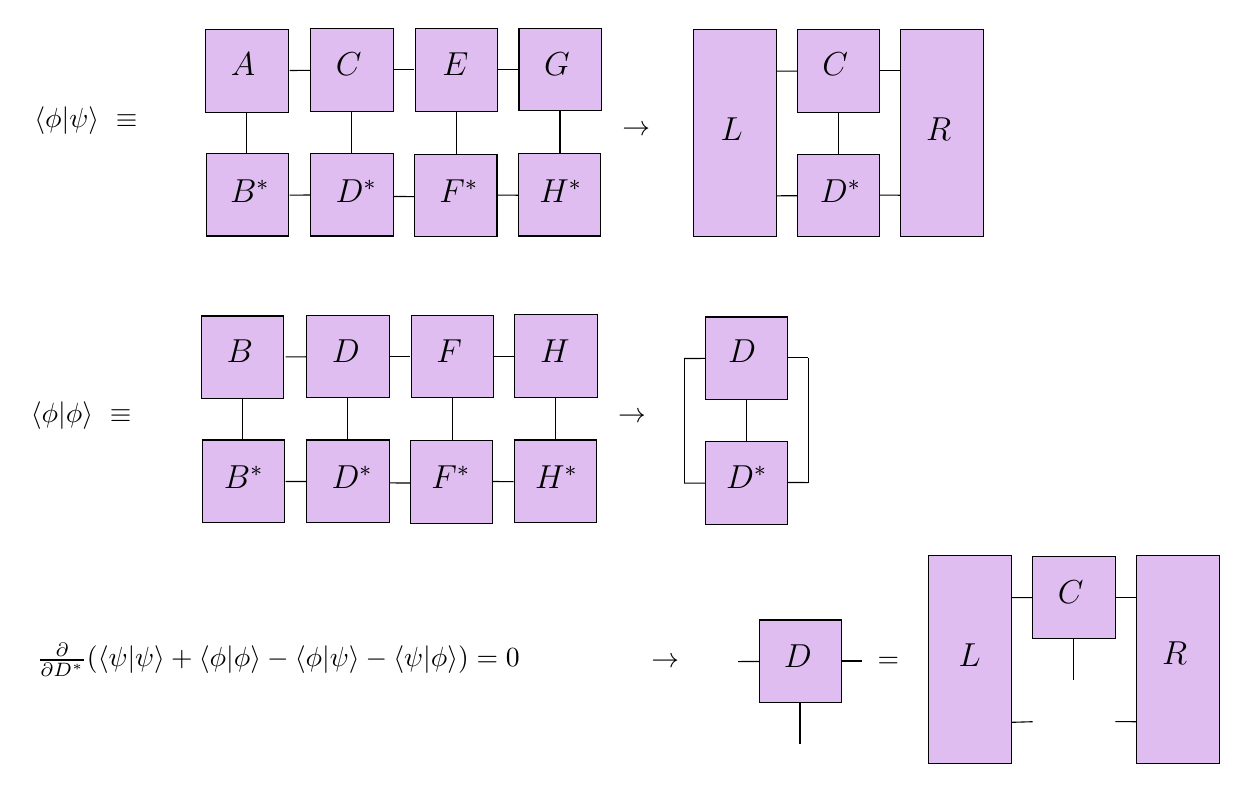
\begin{tikzpicture}[x=0.75pt,y=0.75pt,yscale=-1,xscale=1]
    % uncomment if require: \path (0,372); %set diagram left start at 0, and has height of 372

    % Straight Lines [id:da8829826315861065]
    \draw    (358,225.3) -- (328,225.46) ;
    % Straight Lines [id:da07216189278990481]
    \draw    (357.86,184.1) -- (357.86,205.1) ;
    % Shape: Square [id:dp5599368210722078]
    \draw  [color={rgb, 255:red, 0; green, 0; blue, 0 }  ,draw opacity=1 ][fill={rgb, 255:red, 224; green, 189; blue, 241 }  ,fill opacity=1 ] (338.14,205.43) -- (377.86,205.43) -- (377.86,245.16) -- (338.14,245.16) -- cycle ;
    % Straight Lines [id:da9883461446247077]
    \draw    (358,165.24) -- (328,165.4) ;
    % Shape: Square [id:dp03229039632483821]
    \draw  [color={rgb, 255:red, 0; green, 0; blue, 0 }  ,draw opacity=1 ][fill={rgb, 255:red, 224; green, 189; blue, 241 }  ,fill opacity=1 ] (338.14,145.38) -- (377.86,145.38) -- (377.86,185.1) -- (338.14,185.1) -- cycle ;
    % Straight Lines [id:da8860758652841321]
    \draw    (328,165.4) -- (328,225.46) ;
    % Straight Lines [id:da0050438548697149255]
    \draw    (387.86,165.1) -- (387.86,225.16) ;
    % Straight Lines [id:da6729238405161955]
    \draw    (377.86,165.1) -- (387.86,165.1) ;
    % Straight Lines [id:da4707507889497171]
    \draw    (387.86,225.16) -- (377.86,225.1) ;
    % Straight Lines [id:da828603625691523]
    \draw    (402.33,86.84) -- (372.33,87.01) ;
    % Straight Lines [id:da07556387771217499]
    \draw    (402.2,45.65) -- (402.2,66.65) ;
    % Shape: Square [id:dp012455912523970714]
    \draw  [color={rgb, 255:red, 0; green, 0; blue, 0 }  ,draw opacity=1 ][fill={rgb, 255:red, 224; green, 189; blue, 241 }  ,fill opacity=1 ] (382.47,66.98) -- (422.2,66.98) -- (422.2,106.71) -- (382.47,106.71) -- cycle ;
    % Straight Lines [id:da022178421621197986]
    \draw    (402.33,26.79) -- (372.33,26.95) ;
    % Shape: Square [id:dp985705254035772]
    \draw  [color={rgb, 255:red, 0; green, 0; blue, 0 }  ,draw opacity=1 ][fill={rgb, 255:red, 224; green, 189; blue, 241 }  ,fill opacity=1 ] (382.47,6.92) -- (422.2,6.92) -- (422.2,46.65) -- (382.47,46.65) -- cycle ;
    % Straight Lines [id:da8263634641018831]
    \draw    (422.2,26.65) -- (432.2,26.65) ;
    % Straight Lines [id:da8369258612427866]
    \draw    (432.2,86.71) -- (422.2,86.65) ;
    % Shape: Rectangle [id:dp050508384189636324]
    \draw  [fill={rgb, 255:red, 224; green, 189; blue, 241 }  ,fill opacity=1 ] (332.33,6.71) -- (372.33,6.71) -- (372.33,106.71) -- (332.33,106.71) -- cycle ;
    % Shape: Rectangle [id:dp7109259885356238]
    \draw  [fill={rgb, 255:red, 224; green, 189; blue, 241 }  ,fill opacity=1 ] (432.33,6.71) -- (472.33,6.71) -- (472.33,106.71) -- (432.33,106.71) -- cycle ;
    % Straight Lines [id:da9747415479376995]
    \draw    (383.86,330.1) -- (383.86,351.1) ;
    % Straight Lines [id:da39597903463311757]
    \draw    (384,311.24) -- (354,311.4) ;
    % Shape: Square [id:dp08012456089828257]
    \draw  [color={rgb, 255:red, 0; green, 0; blue, 0 }  ,draw opacity=1 ][fill={rgb, 255:red, 224; green, 189; blue, 241 }  ,fill opacity=1 ] (364.14,291.38) -- (403.86,291.38) -- (403.86,331.1) -- (364.14,331.1) -- cycle ;
    % Straight Lines [id:da11411111658470152]
    \draw    (403.86,311.1) -- (413.86,311.1) ;
    % Straight Lines [id:da6317725964158019]
    \draw    (495.86,340.38) -- (485.86,340.67) ;
    % Straight Lines [id:da39895842721994024]
    \draw    (515.73,299.32) -- (515.73,320.32) ;
    % Straight Lines [id:da43495007267025]
    \draw    (515.86,280.45) -- (485.86,280.62) ;
    % Shape: Square [id:dp288035661343093]
    \draw  [color={rgb, 255:red, 0; green, 0; blue, 0 }  ,draw opacity=1 ][fill={rgb, 255:red, 224; green, 189; blue, 241 }  ,fill opacity=1 ] (496,260.59) -- (535.73,260.59) -- (535.73,300.32) -- (496,300.32) -- cycle ;
    % Straight Lines [id:da43557671150063104]
    \draw    (535.73,280.32) -- (545.73,280.32) ;
    % Straight Lines [id:da33372359877782243]
    \draw    (545.73,340.38) -- (535.73,340.32) ;
    % Shape: Rectangle [id:dp0006495987865049457]
    \draw  [fill={rgb, 255:red, 224; green, 189; blue, 241 }  ,fill opacity=1 ] (445.86,260.38) -- (485.86,260.38) -- (485.86,360.38) -- (445.86,360.38) -- cycle ;
    % Shape: Rectangle [id:dp009958665717864745]
    \draw  [fill={rgb, 255:red, 224; green, 189; blue, 241 }  ,fill opacity=1 ] (545.86,260.38) -- (585.86,260.38) -- (585.86,360.38) -- (545.86,360.38) -- cycle ;
    % Straight Lines [id:da3340208953636794]
    \draw    (168,86.51) -- (138,86.67) ;
    % Straight Lines [id:da4204861203023351]
    \draw    (167.86,45.32) -- (167.86,66.32) ;
    % Shape: Square [id:dp380062386126649]
    \draw  [color={rgb, 255:red, 0; green, 0; blue, 0 }  ,draw opacity=1 ][fill={rgb, 255:red, 224; green, 189; blue, 241 }  ,fill opacity=1 ] (148.14,66.65) -- (187.86,66.65) -- (187.86,106.38) -- (148.14,106.38) -- cycle ;
    % Straight Lines [id:da5661013843550688]
    \draw    (168,26.45) -- (138,26.62) ;
    % Shape: Square [id:dp28420051625087717]
    \draw  [color={rgb, 255:red, 0; green, 0; blue, 0 }  ,draw opacity=1 ][fill={rgb, 255:red, 224; green, 189; blue, 241 }  ,fill opacity=1 ] (148.14,6.59) -- (187.86,6.59) -- (187.86,46.32) -- (148.14,46.32) -- cycle ;
    % Straight Lines [id:da1756070800359002]
    \draw    (187.86,26.32) -- (197.86,26.32) ;
    % Straight Lines [id:da9775208970735725]
    \draw    (197.86,87.38) -- (187.86,87.32) ;
    % Straight Lines [id:da34492543834741896]
    \draw    (117.2,45.65) -- (117.2,66.65) ;
    % Shape: Square [id:dp6337022530370995]
    \draw  [color={rgb, 255:red, 0; green, 0; blue, 0 }  ,draw opacity=1 ][fill={rgb, 255:red, 224; green, 189; blue, 241 }  ,fill opacity=1 ] (97.47,6.92) -- (137.2,6.92) -- (137.2,46.65) -- (97.47,46.65) -- cycle ;
    % Straight Lines [id:da8675115712512742]
    \draw    (218.2,46.32) -- (218.2,67.32) ;
    % Shape: Square [id:dp5736791678261237]
    \draw  [color={rgb, 255:red, 0; green, 0; blue, 0 }  ,draw opacity=1 ][fill={rgb, 255:red, 224; green, 189; blue, 241 }  ,fill opacity=1 ] (198.47,6.59) -- (238.2,6.59) -- (238.2,46.32) -- (198.47,46.32) -- cycle ;
    % Straight Lines [id:da08900027013343159]
    \draw    (238.2,26.32) -- (248.2,26.32) ;
    % Shape: Square [id:dp4779897203177892]
    \draw  [color={rgb, 255:red, 0; green, 0; blue, 0 }  ,draw opacity=1 ][fill={rgb, 255:red, 224; green, 189; blue, 241 }  ,fill opacity=1 ] (97.8,66.65) -- (137.53,66.65) -- (137.53,106.38) -- (97.8,106.38) -- cycle ;
    % Shape: Square [id:dp6648336172525604]
    \draw  [color={rgb, 255:red, 0; green, 0; blue, 0 }  ,draw opacity=1 ][fill={rgb, 255:red, 224; green, 189; blue, 241 }  ,fill opacity=1 ] (198.14,66.98) -- (237.86,66.98) -- (237.86,106.71) -- (198.14,106.71) -- cycle ;
    % Straight Lines [id:da4787017225627974]
    \draw    (247.86,86.71) -- (237.86,86.65) ;
    % Straight Lines [id:da9712231338444757]
    \draw    (268.2,45.98) -- (268.2,66.98) ;
    % Shape: Square [id:dp19331445829840987]
    \draw  [color={rgb, 255:red, 0; green, 0; blue, 0 }  ,draw opacity=1 ][fill={rgb, 255:red, 224; green, 189; blue, 241 }  ,fill opacity=1 ] (248.47,6.26) -- (288.2,6.26) -- (288.2,45.98) -- (248.47,45.98) -- cycle ;
    % Shape: Square [id:dp6363831065636849]
    \draw  [color={rgb, 255:red, 0; green, 0; blue, 0 }  ,draw opacity=1 ][fill={rgb, 255:red, 224; green, 189; blue, 241 }  ,fill opacity=1 ] (248.14,66.65) -- (287.86,66.65) -- (287.86,106.37) -- (248.14,106.37) -- cycle ;
    % Straight Lines [id:da07793992790067761]
    \draw    (166,224.51) -- (136,224.67) ;
    % Straight Lines [id:da8175058506961861]
    \draw    (165.86,183.32) -- (165.86,204.32) ;
    % Shape: Square [id:dp5408057313353591]
    \draw  [color={rgb, 255:red, 0; green, 0; blue, 0 }  ,draw opacity=1 ][fill={rgb, 255:red, 224; green, 189; blue, 241 }  ,fill opacity=1 ] (146.14,204.65) -- (185.86,204.65) -- (185.86,244.38) -- (146.14,244.38) -- cycle ;
    % Straight Lines [id:da7276573039084497]
    \draw    (166,164.45) -- (136,164.62) ;
    % Shape: Square [id:dp5776497888532655]
    \draw  [color={rgb, 255:red, 0; green, 0; blue, 0 }  ,draw opacity=1 ][fill={rgb, 255:red, 224; green, 189; blue, 241 }  ,fill opacity=1 ] (146.14,144.59) -- (185.86,144.59) -- (185.86,184.32) -- (146.14,184.32) -- cycle ;
    % Straight Lines [id:da6186147592870348]
    \draw    (185.86,164.32) -- (195.86,164.32) ;
    % Straight Lines [id:da25392786261407907]
    \draw    (195.86,225.38) -- (185.86,225.32) ;
    % Straight Lines [id:da9103997006668019]
    \draw    (115.2,183.65) -- (115.2,204.65) ;
    % Shape: Square [id:dp6391830498747229]
    \draw  [color={rgb, 255:red, 0; green, 0; blue, 0 }  ,draw opacity=1 ][fill={rgb, 255:red, 224; green, 189; blue, 241 }  ,fill opacity=1 ] (95.47,144.92) -- (135.2,144.92) -- (135.2,184.65) -- (95.47,184.65) -- cycle ;
    % Straight Lines [id:da19950598186645108]
    \draw    (216.2,184.32) -- (216.2,205.32) ;
    % Shape: Square [id:dp36938319273212383]
    \draw  [color={rgb, 255:red, 0; green, 0; blue, 0 }  ,draw opacity=1 ][fill={rgb, 255:red, 224; green, 189; blue, 241 }  ,fill opacity=1 ] (196.47,144.59) -- (236.2,144.59) -- (236.2,184.32) -- (196.47,184.32) -- cycle ;
    % Straight Lines [id:da2738521301765635]
    \draw    (236.2,164.32) -- (246.2,164.32) ;
    % Shape: Square [id:dp38092177783405656]
    \draw  [color={rgb, 255:red, 0; green, 0; blue, 0 }  ,draw opacity=1 ][fill={rgb, 255:red, 224; green, 189; blue, 241 }  ,fill opacity=1 ] (95.8,204.65) -- (135.53,204.65) -- (135.53,244.38) -- (95.8,244.38) -- cycle ;
    % Shape: Square [id:dp9183164595340323]
    \draw  [color={rgb, 255:red, 0; green, 0; blue, 0 }  ,draw opacity=1 ][fill={rgb, 255:red, 224; green, 189; blue, 241 }  ,fill opacity=1 ] (196.14,204.98) -- (235.86,204.98) -- (235.86,244.71) -- (196.14,244.71) -- cycle ;
    % Straight Lines [id:da7996858685122317]
    \draw    (245.86,224.71) -- (235.86,224.65) ;
    % Straight Lines [id:da1705833729460473]
    \draw    (266.2,183.98) -- (266.2,204.98) ;
    % Shape: Square [id:dp08053850547950203]
    \draw  [color={rgb, 255:red, 0; green, 0; blue, 0 }  ,draw opacity=1 ][fill={rgb, 255:red, 224; green, 189; blue, 241 }  ,fill opacity=1 ] (246.47,144.26) -- (286.2,144.26) -- (286.2,183.98) -- (246.47,183.98) -- cycle ;
    % Shape: Square [id:dp6783705440409395]
    \draw  [color={rgb, 255:red, 0; green, 0; blue, 0 }  ,draw opacity=1 ][fill={rgb, 255:red, 224; green, 189; blue, 241 }  ,fill opacity=1 ] (246.14,204.65) -- (285.86,204.65) -- (285.86,244.37) -- (246.14,244.37) -- cycle ;

    % Text Node
    \draw (347,216) node [anchor=north west][inner sep=0.75pt]  [font=\large]  {$D^{*}$};
    % Text Node
    \draw (348,155) node [anchor=north west][inner sep=0.75pt]  [font=\large]  {$D$};
    % Text Node
    \draw (12,184.78) node [anchor=north west][inner sep=0.75pt]    {$\langle \phi |\phi \rangle \ \equiv $};
    % Text Node
    \draw (392.2,78) node [anchor=north west][inner sep=0.75pt]  [font=\large]  {$D^{*}$};
    % Text Node
    \draw (393.33,17) node [anchor=north west][inner sep=0.75pt]  [font=\large]  {$C$};
    % Text Node
    \draw (13.67,42.99) node [anchor=north west][inner sep=0.75pt]    {$\langle \phi | \psi \rangle \ \equiv $};
    % Text Node
    \draw (344.33,48.11) node [anchor=north west][inner sep=0.75pt]  [font=\large]  {$L$};
    % Text Node
    \draw (443.33,48.11) node [anchor=north west][inner sep=0.75pt]  [font=\large]  {$R$};
    % Text Node
    \draw (15,301) node [anchor=north west][inner sep=0.75pt]    {$\frac{\partial }{\partial D^{*}}( \langle \psi |\psi \rangle +\langle \phi |\phi \rangle -\langle \phi |\psi \rangle -\langle \psi |\phi \rangle ) =0$};
    % Text Node
    \draw (374.86,302) node [anchor=north west][inner sep=0.75pt]  [font=\large]  {$D$};
    % Text Node
    \draw (506.86,271) node [anchor=north west][inner sep=0.75pt]  [font=\large]  {$C$};
    % Text Node
    \draw (459,301.78) node [anchor=north west][inner sep=0.75pt]  [font=\large]  {$L$};
    % Text Node
    \draw (557,300.78) node [anchor=north west][inner sep=0.75pt]  [font=\large]  {$R$};
    % Text Node
    \draw (420,308) node [anchor=north west][inner sep=0.75pt]    {$=$};
    % Text Node
    \draw (158.86,78) node [anchor=north west][inner sep=0.75pt]  [font=\large]  {$D^{*}$};
    % Text Node
    \draw (159,17) node [anchor=north west][inner sep=0.75pt]  [font=\large]  {$C$};
    % Text Node
    \draw (108.33,17) node [anchor=north west][inner sep=0.75pt]  [font=\large]  {$A$};
    % Text Node
    \draw (210.33,17) node [anchor=north west][inner sep=0.75pt]  [font=\large]  {$E$};
    % Text Node
    \draw (108,78) node [anchor=north west][inner sep=0.75pt]  [font=\large]  {$B^{*}$};
    % Text Node
    \draw (208.86,78) node [anchor=north west][inner sep=0.75pt]  [font=\large]  {$F^{*}$};
    % Text Node
    \draw (259.33,17) node [anchor=north west][inner sep=0.75pt]  [font=\large]  {$G$};
    % Text Node
    \draw (257,78) node [anchor=north west][inner sep=0.75pt]  [font=\large]  {$H^{*}$};
    % Text Node
    \draw (297,52) node [anchor=north west][inner sep=0.75pt]    {$\rightarrow $};
    % Text Node
    \draw (156.86,216) node [anchor=north west][inner sep=0.75pt]  [font=\large]  {$D^{*}$};
    % Text Node
    \draw (157,155) node [anchor=north west][inner sep=0.75pt]  [font=\large]  {$D$};
    % Text Node
    \draw (106.33,155) node [anchor=north west][inner sep=0.75pt]  [font=\large]  {$B$};
    % Text Node
    \draw (207.33,155) node [anchor=north west][inner sep=0.75pt]  [font=\large]  {$F$};
    % Text Node
    \draw (105,216) node [anchor=north west][inner sep=0.75pt]  [font=\large]  {$B^{*}$};
    % Text Node
    \draw (205,216) node [anchor=north west][inner sep=0.75pt]  [font=\large]  {$F^{*}$};
    % Text Node
    \draw (257.33,155) node [anchor=north west][inner sep=0.75pt]  [font=\large]  {$H$};
    % Text Node
    \draw (255,216) node [anchor=north west][inner sep=0.75pt]  [font=\large]  {$H^{*}$};
    % Text Node
    \draw (295,190) node [anchor=north west][inner sep=0.75pt]    {$\rightarrow $};
    % Text Node
    \draw (311,308) node [anchor=north west][inner sep=0.75pt]    {$\rightarrow $};


  \end{tikzpicture}
  \caption{Diagrammatic representation of one step of the simplification algorithm for MPS.}\label{fig:mps simplification}
\end{figure}

We can extend this algorithm to the approximation of a linear combination of states, i.e., to solve the problem

\begin{eqnarray}
  \mathrm{argmin}_{\phi\in\mathrm{MPS}}\left\Vert\phi- \sum_{n=1}^{N}\alpha_n\psi_n\right\Vert^2.
\end{eqnarray}
In this case we have an antilinear form for every scalar product $\langle\phi|\psi_n\rangle$, and the solution is a weighted linear combination of the solution for each state
\begin{eqnarray}
  D^i_{\alpha,\beta} = \sum_{n=1}^{N}\alpha_n U_{\alpha\beta}^{(n)i}.
\end{eqnarray}



\section{Time step limitation in Runge-Kutta methods} \label{app: step size}

In the imaginary-time evolution Runge-Kutta methods in Section\ \ref{sec:ImaginaryTimeEvolution}, correctly choosing the step size $\Delta\beta$ is key to optimize the convergence to the ground state. This convergence is determined by the contraction ratio $r_m$,

\begin{eqnarray} \label{eq: contraction ratio}
  r_m = \frac{\lambda_m(\beta,E_m)}{\lambda_0(\beta,E_0)}, \quad m > 0,
\end{eqnarray}
where $\lambda(\Delta\beta,E_n)$ is the eigenvalue of the Runge-Kutta method for the $n$th energy level and step size $\Delta\beta$. The smaller this value, the faster the component of the corresponding $m$-th energy level goes to zero. The form of the contraction ratio depends on how the imaginary-time evolution method approximates the evolution operator, so the optimum $\Delta\beta$ varies for each numerical method. To study this, let us plot the contraction ratios of the energy levels corresponding to the quantum harmonic oscillator \eqref{eq: ho} 3-qubit discretization for a range of values of $\Delta\beta$. We represent them for $r_m \leq |1|$, as outside this interval convergence is not assured. We observe that higher-order methods approximate better the exact theoretical evolution, especially for the smallest $\Delta\beta s$, as expected due to the smaller global error associated with them. However, although the Euler method fails to reproduce the behavior of the evolution for larger values of $\Delta\beta$, it can achieve smaller contraction ratios and consequently faster convergence.

\begin{figure}[H]
  \centering
  \centering
  \includegraphics[width=0.7\textwidth]{figures/contraction_ratio.pdf}
  \caption{Contraction ratio $r_m$ of the one-dimensional quantum harmonic oscillator \eqref{eq: ho} 3-qubit discretization for $\Delta\beta \in [0,1]$. The different line styles correspond to the used methods: theoretical evolution (solid), Euler (dash-dotted), improved Euler (dotted), and Runge-Kutta (dashed).}
  \label{fig:contraction ratio}
\end{figure}

Not only the step size $\Delta\beta$, but also the initial state $\psi(\beta_0)$, plays a key role in the convergence. For $c_0 = \langle \varphi_0 | \psi(\beta_0)\rangle = 0$, the state cannot evolve to the ground state, so we need to make sure that the initial state has $c_0 \neq 0$. In addition, if the ground state has some $c_i =0, \ i\neq 0$, their corresponding contraction ratios will not be considered for the computation of $\Delta\beta_\mathrm{opt}$. Thus, the optimum step size will depend on the initial state.

In general, the spectrum of the problem that we are aiming to solve is unknown, so we cannot compute the contraction ratios or the $c_n$ coefficients. In these cases, we will use a minimization algorithm that finds the optimum step size according to a certain figure of merit acting as cost function. This algorithm requires applying the method as many times as optimization steps necessary to reach the optimum step size but allows us to find a better approximation than simple inspection in fewer executions of the numerical method when a good initial approximation of $\Delta\beta_\mathrm{opt}$ is used.

\section{Density matrix renormalization group} \label{app: DMRG}

The density matrix renormalization group (DMRG) is a numerical algorithm originally developed for the study of the low-energy physics of quantum many-body physics\ \cite{White1992, White1993}. This approach was adapted to the formalism of MPS\ \cite{Verstraete2004b, Schollwoeck2005, Schollwoeck2011}, extending it to a quantum information perspective. Since then, it constitutes one of the most important MPS algorithms, as it performs an iterative variational optimization of the MPS. This optimization procedure is mainly used to obtain the ground state of the Hamiltonian of a quantum many-body system. Other applications are the computation of excited states\ \cite{Chandross1999, Baiardi2022}, dynamical systems\ \cite{Jeckelmann2002}, or the real-time evolution of quantum systems via time-dependent DMRG (tDMRG)\ \cite{Daley2004, White2004, Schollwoeck2006}.

The DMRG algorithm approximates the dominant eigenvector of the Hamiltonian matrix $H$, where the eigenvector is written as an MPS. To perform this it uses the variational method, i.e., for a given quantum state $\ket{\psi}$,

\begin{eqnarray}
  E_0 \leq \frac{\bra{\psi}H\ket{\psi}}{\langle \psi | \psi\rangle},
\end{eqnarray}
where $E_0$ is the ground state energy and the inequality is saturated for $\ket{\psi} = \ket{\psi_0}$, where $\ket{\psi_0}$ is the ground state of $H$. The variation of the MPS is performed locally on each site $M$, such that at each step the energy $E$
\begin{eqnarray}
  E = \frac{\bra{\psi^{[M]}}H_M\ket{\psi^{[M]}}}{\langle \psi^{[M]} |N_M| \psi^{[M]}\rangle},
\end{eqnarray}
where $\ket{\psi^{[M]}}$ is the MPS rewritten as a tensor, and $H_M$ and $N_M$ are the Hamiltonian and normalization matrices, that correspond to the environments of tensors $\psi^{[M]}$ and $\psi^*{^{[M]}}$ for $\bra{\psi}H\ket{\psi}$ and $\langle \psi | \psi\rangle$\ \cite{Orus2014}. Then, we solve the minimization problem for site $M$ at each step given by

\begin{eqnarray}
  \min_{\psi^{[M]}} \left(\bra{\psi^{[M]}}H_M\ket{\psi^{[M]}}-\lambda\bra{\psi^{[M]}}N_M\ket{\psi^{[M]}}\right).
\end{eqnarray}
By taking the derivative of the previous expression with respect to $\psi^{*^{[M]}}$ we obtain that the minimization problem is equivalent to the following generalized eigenvalue problem

\begin{eqnarray}
  H_M |\psi^{[M]}\rangle = \lambda N_M  |\psi^{[M]}\rangle.
\end{eqnarray}
Therefore, we need to solve a system of equations at each step to obtain the optimized site. This process is iteratively repeated on each site on the MPS, and several sweeps of the MPS are performed until convergence, for which $|\psi\rangle$ is a high precision approximation of the dominant eigenvector of $H$.

\section{Interpolation}
\label{sec:interpolation}

The previous description is a discrete approximation of continuous functions and operators. We can increase its precision  using interpolation. For functions that meet the requirements for the spectral method, we can arbitrarily increase this precision---up to $O(e^{-r2^n}), $ for analytic functions, where $r$ is a problem-dependent constant\ \cite{GarciaMolina2022}---using Fourier interpolation. This technique reconstructs the original continuous, bandwidth-limited, infinitely differentiable function from the momentum space discrete approximation
\begin{eqnarray}
  \label{eq:continuous-position}
  f(\mathbf{x}) \propto \sum_{\lbrace s_i\rbrace} e^{-ip_{\bm{s}} x} \langle{\bm{s}|\bm{\mathcal{F}} |f^{(n)}}\rangle.
\end{eqnarray}.

We can also use the finite difference method to perform the interpolation. We can reconstruct the $(n+1)$-qubit function from the $n$-qubit one by dividing the spatial discretization step $\Delta x_i$ by two, and approximating the middle points as
\begin{eqnarray}
  f(\mathbf{x} + \Delta \mathbf{x}/2) &\approx f(\mathbf{x}) + \frac{\Delta \mathbf{x}}{2} \nabla f(\bm{x+ \Delta \mathbf{x}/2}) \\
                                      &\approx f(\mathbf{x}) + \frac{f(\mathbf{x} + \Delta\mathbf{x})-f(\mathbf{x})}{2},
\end{eqnarray}
where $\Delta \mathbf{x} = (\Delta x_1,\dots, \Delta x_d)$.

\section{Extension of the global optimization to other PDEs} \label{app: source PDEs}

The global optimization methods can solve another type of PDEs as long as we can rewrite them in the form of a cost function that will lead to the solution. A possible application is the resolution of PDEs with a source term $g(x)$,
\begin{eqnarray}\label{eq: source PDE}
  Df(x) = g(x), \quad f(x), g(x) \in \mathbb{C}^N.
\end{eqnarray}
We solve \eqref{eq: source PDE} by minimizing the cost functional $C[f]$,
\begin{eqnarray} \label{eq: cost source PDE}
  C[f] = || Df(x)-g(x)||^2.
\end{eqnarray}
The gradient descent algorithm\ \ref{sec:gradient descent} then follows the optimization path
\begin{eqnarray}\label{eq: descent source eq}
  f_{n+1} = f_n + \Delta\beta D^\dagger(Df- g) = f_n + \Delta\beta D^\dagger w,
\end{eqnarray}
and using the optimum $\Delta\beta$ for each step,
\begin{eqnarray} \label{eq: step source eq}
  \Delta\beta_\mathrm{opt} = - \frac{\langle w | D D^\dagger | w\rangle}{\langle w | D D^\dagger D D^\dagger |w\rangle}.
\end{eqnarray}

The efficient resolution of PDEs with source terms is key, due to the multiple applications of such equations. Some important source PDEs are Poisson's equation and the heat equation, which have many applications beyond their original use, as many models can be reduced to them. An interesting example is the use of the heat equation in finance, as the Black-Scholes equation\ \cite{Black1973} can be expressed in terms of it.

\section*{References}

\bibliographystyle{unsrt}
\bibliography{my_bibliography}


\end{document}
